%\documentclass[11pt, a4paper,dalthesis]{report}    % final 
%\documentclass[11pt,a4paper,dalthesis]{report}
%\documentclass[11pt,a4paper,dalthesis]{book}

\documentclass[11pt,a4paper,titlepage,oneside,openany]{article}

\pagestyle{plain}
%\renewcommand{\baselinestretch}{1.7}

\usepackage{setspace}
%\singlespacing
\onehalfspacing
%\doublespacing
%\setstretch{1.1}

\usepackage{amsmath}
\usepackage{amssymb}
\usepackage{amsthm}
\usepackage{multicol}

\usepackage[margin=3cm]{geometry}
\usepackage{graphicx,psfrag}%\usepackage{hyperref}
\usepackage[small]{caption}
\usepackage{subfig}

\usepackage{algorithm}
\usepackage{algorithmic}
\newcommand{\theHalgorithm}{\arabic{algorithm}}

\usepackage{varioref} %NB: FIGURE LABELS MUST ALWAYS COME DIRECTLY AFTER CAPTION!!!
%\newcommand{\vref}{\ref}

\usepackage{index}
\makeindex
\newindex{sym}{adx}{and}{Symbol Index}
%\newcommand{\symindex}{\index[sym]}
%\newcommand{\symindex}[1]{\index[sym]{#1}\hfill}
\newcommand{\symindex}[1]{\index[sym]{#1}}

%\usepackage[breaklinks,dvips]{hyperref}%Always put after varioref, or you'll get nested section headings
%Make sure this is after index package too!
%\hypersetup{colorlinks=false,breaklinks=true}
%\hypersetup{colorlinks=false,breaklinks=true,pdfborder={0 0 0.15}}


%\usepackage{breakurl}

\graphicspath{{./images/}}

\usepackage[subfigure]{tocloft}%For table of contents
\setlength{\cftfignumwidth}{3em}

\input{longdiv}
\usepackage{wrapfig}


%\usepackage{index}
%\makeindex
%\usepackage{makeidx}

%\usepackage{lscape}
\usepackage{pdflscape}
\usepackage{multicol}

\usepackage[utf8]{inputenc}

%\usepackage{fullpage}

%Compulsory packages for the PhD in UL:
%\usepackage{UL Thesis}
\usepackage{natbib}

%\numberwithin{equation}{section}
\numberwithin{equation}{section}
\numberwithin{algorithm}{section}
\numberwithin{figure}{section}
\numberwithin{table}{section}
%\newcommand{\vec}[1]{\ensuremath{\math{#1}}}

%\linespread{1.6} %for double line spacing

\usepackage{afterpage}%fingers crossed

\newtheorem{thm}{Theorem}[section]
\newtheorem{defin}{Definition}[section]
\newtheorem{cor}[thm]{Corollary}
\newtheorem{lem}[thm]{Lemma}

%\newcommand{\dbar}{{\mkern+3mu\mathchar'26\mkern-12mu d}}
\newcommand{\dbar}{{\mkern+3mu\mathchar'26\mkern-12mud}}

\newcommand{\bbSigma}{{\mkern+8mu\mathsf{\Sigma}\mkern-9mu{\Sigma}}}
\newcommand{\thrfor}{{\Rightarrow}}

\newcommand{\mb}{\mathbb}
\newcommand{\bx}{\vec{x}}
\newcommand{\bxi}{\boldsymbol{\xi}}
\newcommand{\bdeta}{\boldsymbol{\eta}}
\newcommand{\bldeta}{\boldsymbol{\eta}}
\newcommand{\bgamma}{\boldsymbol{\gamma}}
\newcommand{\bTheta}{\boldsymbol{\Theta}}
\newcommand{\balpha}{\boldsymbol{\alpha}}
\newcommand{\bmu}{\boldsymbol{\mu}}
\newcommand{\bnu}{\boldsymbol{\nu}}
\newcommand{\bsigma}{\boldsymbol{\sigma}}
\newcommand{\bdiff}{\boldsymbol{\partial}}

\newcommand{\tomega}{\widetilde{\omega}}
\newcommand{\tbdeta}{\widetilde{\bdeta}}
\newcommand{\tbxi}{\widetilde{\bxi}}



\newcommand{\wv}{\vec{w}}

\newcommand{\ie}{i.e. }
\newcommand{\eg}{e.g. }
\newcommand{\etc}{etc}

\newcommand{\viceversa}{vice versa}
\newcommand{\FT}{\mathcal{F}}
\newcommand{\IFT}{\mathcal{F}^{-1}}
%\renewcommand{\vec}[1]{\boldsymbol{#1}}
\renewcommand{\vec}[1]{\mathbf{#1}}
\newcommand{\anged}[1]{\langle #1 \rangle}
\newcommand{\grv}[1]{\grave{#1}}
\newcommand{\asinh}{\sinh^{-1}}

\newcommand{\sgn}{\text{sgn}}
\newcommand{\morm}[1]{|\det #1 |}

\newcommand{\galpha}{\grv{\alpha}}
\newcommand{\gbeta}{\grv{\beta}}
%\newcommand{\rnlessO}{\mb{R}^n \setminus \vec{0}}
\usepackage{listings}
\usepackage{arydshln}

\interfootnotelinepenalty=10000

\newcommand{\sectionline}{%
  \nointerlineskip \vspace{\baselineskip}%
  \hspace{\fill}\rule{0.5\linewidth}{.7pt}\hspace{\fill}%
  \par\nointerlineskip \vspace{\baselineskip}
}

\renewcommand{\labelenumii}{\roman{enumii})}

\begin{document}

\begin{landscape}
\begin{center}
  \textbf{Tutorial Sheet 3}
\end{center}


Let the function $f$ be given by the rule $f(x)=x-\log(x)-\sqrt{2}$.
\begin{enumerate}

\item
  Using intervals of $0.5$, evaluate $f$ from $x=0.5$ to $x=3$ and hence sketch the graph of $f(x)$ over this interval.

\item 
  Use the bisection method to estimate the root of $f(x)$ in the interval $[0.5,3]$. Start with an interval of length $1$ and iterate until the size of the interval is less than $0.01$.

\item
  Given that $f'(x)=1-\frac{1}{x}$, use the Newton-Raphson method to estimate the root of $f(x)$ in the interval $[0.5,3]$. Use an integer as an initial estimate for the root. \hfill Ans $\cong 2.20489216557483$
\\
\\
\begin{tabular}{|l|c|c:c:c:c:c:c:c:c:c|c|c:c:c:c:c:c:c:c:c|c|c:c:c:c:c:c:c:c:c|c|c:c:c:c:c:c:c:c:c|}\hline
$n$ & \ & \multicolumn{9}{c|}{$x_n$} & \ & \multicolumn{9}{c|}{$f(x_n)$} & \ & \multicolumn{9}{c|}{$f'(x_n)$} & \ & \multicolumn{9}{c|}{${f(x_n)}/{f'(x_n)}$} \\ \hline
$0$ & \ &
\hspace{0.4em} & \hspace{0.4em} & $\cdot$ & \hspace{0.4em} & \hspace{0.4em} & \hspace{0.4em} & \hspace{0.4em} & \hspace{0.4em} & \hspace{0.4em}  & \ &
\hspace{0.4em} & \hspace{0.4em} & $\cdot$ & \hspace{0.4em} & \hspace{0.4em} & \hspace{0.4em} & \hspace{0.4em} & \hspace{0.4em} & \hspace{0.4em}  & \ &
\hspace{0.4em} & \hspace{0.4em} & $\cdot$ & \hspace{0.4em} & \hspace{0.4em} & \hspace{0.4em} & \hspace{0.4em} & \hspace{0.4em} & \hspace{0.4em}  & \ &
\hspace{0.4em} & \hspace{0.4em} & $\cdot$ & \hspace{0.4em} & \hspace{0.4em} & \hspace{0.4em} & \hspace{0.4em} & \hspace{0.4em} & \hspace{0.4em}  \\ \hline
$1$ & \ &
\hspace{0.4em} & \hspace{0.4em} & $\cdot$ & \hspace{0.4em} & \hspace{0.4em} & \hspace{0.4em} & \hspace{0.4em} & \hspace{0.4em} & \hspace{0.4em}  & \ &
\hspace{0.4em} & \hspace{0.4em} & $\cdot$ & \hspace{0.4em} & \hspace{0.4em} & \hspace{0.4em} & \hspace{0.4em} & \hspace{0.4em} & \hspace{0.4em}  & \ &
\hspace{0.4em} & \hspace{0.4em} & $\cdot$ & \hspace{0.4em} & \hspace{0.4em} & \hspace{0.4em} & \hspace{0.4em} & \hspace{0.4em} & \hspace{0.4em}  & \ &
\hspace{0.4em} & \hspace{0.4em} & $\cdot$ & \hspace{0.4em} & \hspace{0.4em} & \hspace{0.4em} & \hspace{0.4em} & \hspace{0.4em} & \hspace{0.4em}  \\ \hline
$2$ & \ &
\hspace{0.4em} & \hspace{0.4em} & $\cdot$ & \hspace{0.4em} & \hspace{0.4em} & \hspace{0.4em} & \hspace{0.4em} & \hspace{0.4em} & \hspace{0.4em}  & \ &
\hspace{0.4em} & \hspace{0.4em} & $\cdot$ & \hspace{0.4em} & \hspace{0.4em} & \hspace{0.4em} & \hspace{0.4em} & \hspace{0.4em} & \hspace{0.4em}  & \ &
\hspace{0.4em} & \hspace{0.4em} & $\cdot$ & \hspace{0.4em} & \hspace{0.4em} & \hspace{0.4em} & \hspace{0.4em} & \hspace{0.4em} & \hspace{0.4em}  & \ &
\hspace{0.4em} & \hspace{0.4em} & $\cdot$ & \hspace{0.4em} & \hspace{0.4em} & \hspace{0.4em} & \hspace{0.4em} & \hspace{0.4em} & \hspace{0.4em}  \\ \hline
$3$ & \ &
\hspace{0.4em} & \hspace{0.4em} & $\cdot$ & \hspace{0.4em} & \hspace{0.4em} & \hspace{0.4em} & \hspace{0.4em} & \hspace{0.4em} & \hspace{0.4em}  & \ &
\hspace{0.4em} & \hspace{0.4em} & $\cdot$ & \hspace{0.4em} & \hspace{0.4em} & \hspace{0.4em} & \hspace{0.4em} & \hspace{0.4em} & \hspace{0.4em}  & \ &
\hspace{0.4em} & \hspace{0.4em} & $\cdot$ & \hspace{0.4em} & \hspace{0.4em} & \hspace{0.4em} & \hspace{0.4em} & \hspace{0.4em} & \hspace{0.4em}  & \ &
\hspace{0.4em} & \hspace{0.4em} & $\cdot$ & \hspace{0.4em} & \hspace{0.4em} & \hspace{0.4em} & \hspace{0.4em} & \hspace{0.4em} & \hspace{0.4em}  \\ \hline
$4$ & \ &
\hspace{0.4em} & \hspace{0.4em} & $\cdot$ & \hspace{0.4em} & \hspace{0.4em} & \hspace{0.4em} & \hspace{0.4em} & \hspace{0.4em} & \hspace{0.4em}  & \ &
\hspace{0.4em} & \hspace{0.4em} & $\cdot$ & \hspace{0.4em} & \hspace{0.4em} & \hspace{0.4em} & \hspace{0.4em} & \hspace{0.4em} & \hspace{0.4em}  & \ &
\hspace{0.4em} & \hspace{0.4em} & $\cdot$ & \hspace{0.4em} & \hspace{0.4em} & \hspace{0.4em} & \hspace{0.4em} & \hspace{0.4em} & \hspace{0.4em}  & \ &
\hspace{0.4em} & \hspace{0.4em} & $\cdot$ & \hspace{0.4em} & \hspace{0.4em} & \hspace{0.4em} & \hspace{0.4em} & \hspace{0.4em} & \hspace{0.4em}  \\ \hline
%$$ & \ &
%\ & \ & $\cdot$ & \ & \ & \ & \ & \ & \  & \ &
%\ & \ & $\cdot$ & \ & \ & \ & \ & \ & \  \\ \hline
\end{tabular}
\\
\item
  Use Newton's Method to find a root of $f(x)$ starting with an initial guess of $0.5$. \hfill Ans $\cong 0.342380252644745$
\\
\\
\begin{tabular}{|l|c|c:c:c:c:c:c:c:c:c|c|c:c:c:c:c:c:c:c:c|c|c:c:c:c:c:c:c:c:c|c|c:c:c:c:c:c:c:c:c|}\hline
$n$ & \ & \multicolumn{9}{c|}{$x_n$} & \ & \multicolumn{9}{c|}{$f(x_n)$} & \ & \multicolumn{9}{c|}{$f'(x_n)$} & \ & \multicolumn{9}{c|}{${f(x_n)}/{f'(x_n)}$} \\ \hline
$0$ & \ &
\hspace{0.4em} & \hspace{0.4em} & $\cdot$ & \hspace{0.4em} & \hspace{0.4em} & \hspace{0.4em} & \hspace{0.4em} & \hspace{0.4em} & \hspace{0.4em}  & \ &
\hspace{0.4em} & \hspace{0.4em} & $\cdot$ & \hspace{0.4em} & \hspace{0.4em} & \hspace{0.4em} & \hspace{0.4em} & \hspace{0.4em} & \hspace{0.4em}  & \ &
\hspace{0.4em} & \hspace{0.4em} & $\cdot$ & \hspace{0.4em} & \hspace{0.4em} & \hspace{0.4em} & \hspace{0.4em} & \hspace{0.4em} & \hspace{0.4em}  & \ &
\hspace{0.4em} & \hspace{0.4em} & $\cdot$ & \hspace{0.4em} & \hspace{0.4em} & \hspace{0.4em} & \hspace{0.4em} & \hspace{0.4em} & \hspace{0.4em}  \\ \hline
$1$ & \ &
\hspace{0.4em} & \hspace{0.4em} & $\cdot$ & \hspace{0.4em} & \hspace{0.4em} & \hspace{0.4em} & \hspace{0.4em} & \hspace{0.4em} & \hspace{0.4em}  & \ &
\hspace{0.4em} & \hspace{0.4em} & $\cdot$ & \hspace{0.4em} & \hspace{0.4em} & \hspace{0.4em} & \hspace{0.4em} & \hspace{0.4em} & \hspace{0.4em}  & \ &
\hspace{0.4em} & \hspace{0.4em} & $\cdot$ & \hspace{0.4em} & \hspace{0.4em} & \hspace{0.4em} & \hspace{0.4em} & \hspace{0.4em} & \hspace{0.4em}  & \ &
\hspace{0.4em} & \hspace{0.4em} & $\cdot$ & \hspace{0.4em} & \hspace{0.4em} & \hspace{0.4em} & \hspace{0.4em} & \hspace{0.4em} & \hspace{0.4em}  \\ \hline
$2$ & \ &
\hspace{0.4em} & \hspace{0.4em} & $\cdot$ & \hspace{0.4em} & \hspace{0.4em} & \hspace{0.4em} & \hspace{0.4em} & \hspace{0.4em} & \hspace{0.4em}  & \ &
\hspace{0.4em} & \hspace{0.4em} & $\cdot$ & \hspace{0.4em} & \hspace{0.4em} & \hspace{0.4em} & \hspace{0.4em} & \hspace{0.4em} & \hspace{0.4em}  & \ &
\hspace{0.4em} & \hspace{0.4em} & $\cdot$ & \hspace{0.4em} & \hspace{0.4em} & \hspace{0.4em} & \hspace{0.4em} & \hspace{0.4em} & \hspace{0.4em}  & \ &
\hspace{0.4em} & \hspace{0.4em} & $\cdot$ & \hspace{0.4em} & \hspace{0.4em} & \hspace{0.4em} & \hspace{0.4em} & \hspace{0.4em} & \hspace{0.4em}  \\ \hline
$3$ & \ &
\hspace{0.4em} & \hspace{0.4em} & $\cdot$ & \hspace{0.4em} & \hspace{0.4em} & \hspace{0.4em} & \hspace{0.4em} & \hspace{0.4em} & \hspace{0.4em}  & \ &
\hspace{0.4em} & \hspace{0.4em} & $\cdot$ & \hspace{0.4em} & \hspace{0.4em} & \hspace{0.4em} & \hspace{0.4em} & \hspace{0.4em} & \hspace{0.4em}  & \ &
\hspace{0.4em} & \hspace{0.4em} & $\cdot$ & \hspace{0.4em} & \hspace{0.4em} & \hspace{0.4em} & \hspace{0.4em} & \hspace{0.4em} & \hspace{0.4em}  & \ &
\hspace{0.4em} & \hspace{0.4em} & $\cdot$ & \hspace{0.4em} & \hspace{0.4em} & \hspace{0.4em} & \hspace{0.4em} & \hspace{0.4em} & \hspace{0.4em}  \\ \hline
$4$ & \ &
\hspace{0.4em} & \hspace{0.4em} & $\cdot$ & \hspace{0.4em} & \hspace{0.4em} & \hspace{0.4em} & \hspace{0.4em} & \hspace{0.4em} & \hspace{0.4em}  & \ &
\hspace{0.4em} & \hspace{0.4em} & $\cdot$ & \hspace{0.4em} & \hspace{0.4em} & \hspace{0.4em} & \hspace{0.4em} & \hspace{0.4em} & \hspace{0.4em}  & \ &
\hspace{0.4em} & \hspace{0.4em} & $\cdot$ & \hspace{0.4em} & \hspace{0.4em} & \hspace{0.4em} & \hspace{0.4em} & \hspace{0.4em} & \hspace{0.4em}  & \ &
\hspace{0.4em} & \hspace{0.4em} & $\cdot$ & \hspace{0.4em} & \hspace{0.4em} & \hspace{0.4em} & \hspace{0.4em} & \hspace{0.4em} & \hspace{0.4em}  \\ \hline
$5$ & \ &
\hspace{0.4em} & \hspace{0.4em} & $\cdot$ & \hspace{0.4em} & \hspace{0.4em} & \hspace{0.4em} & \hspace{0.4em} & \hspace{0.4em} & \hspace{0.4em}  & \ &
\hspace{0.4em} & \hspace{0.4em} & $\cdot$ & \hspace{0.4em} & \hspace{0.4em} & \hspace{0.4em} & \hspace{0.4em} & \hspace{0.4em} & \hspace{0.4em}  & \ &
\hspace{0.4em} & \hspace{0.4em} & $\cdot$ & \hspace{0.4em} & \hspace{0.4em} & \hspace{0.4em} & \hspace{0.4em} & \hspace{0.4em} & \hspace{0.4em}  & \ &
\hspace{0.4em} & \hspace{0.4em} & $\cdot$ & \hspace{0.4em} & \hspace{0.4em} & \hspace{0.4em} & \hspace{0.4em} & \hspace{0.4em} & \hspace{0.4em}  \\ \hline
%$$ & \ &
%\ & \ & $\cdot$ & \ & \ & \ & \ & \ & \  & \ &
%\ & \ & $\cdot$ & \ & \ & \ & \ & \ & \  \\ \hline
\end{tabular}

\end{enumerate}

\end{landscape}

\pagebreak

\begin{center}
  \textbf{Tutorial Sheet 4}
\end{center}

Derivatives of polynomials 
$f(x)=x^n,\quad  f'(x)=n x^{n-1}$ \qquad
$f(x)=C,  f'(x)=0$\\
$f(x)=A g(x) + B h(x),  f'(x)=A g'(x) + B h'(x)$
\begin{enumerate}
\item Find the derivatives of the following polynomials
  \begin{multicols}{2}
    \begin{enumerate}
    \item $x^2+x+1$\hfill Ans. $2x+1$
    \item $3x^2-9x+4$\hfill Ans. $6x-9$
    \item $\frac{1}{x}$\hfill Ans. $-\frac{1}{x^2}$
    \item $\frac{4}{x^3}$\hfill Ans. $-\frac{12}{x^4}$
    \item $\frac{10}{x^4}-\frac{3}{x^5}$\hfill Ans. $\frac{15}{x^6}-\frac{40}{x^5}$
    \item $\frac{x^2}{3}+\frac{4x}{5}$\hfill Ans. $\frac{2x}{3}+\frac{4}{5}$
    \item $\sqrt{x}$\hfill Ans. $\frac{1}{2\sqrt{x}}$
    \item $11x^7-7x^{11}+12$\hfill Ans. $77(x^6-x^{10})$
    \item $7x^4-x^3+x(x-1)$ \\ \hfill Ans. $28x^3-3x^2+2x-1$
    \end{enumerate}
  \end{multicols}

\item
  The Newton-Heron method to compute $\sqrt[k]{D}$ starts from an initial guess $x_0$ and updates according to the rule
  \begin{equation*}
    x_{n+1}= \left( \frac{k-1}{k}\right)x_n + \frac{D}{k x_n^{k-1}}
  \end{equation*}
  Use Newton's method to derive this formula by considering the problem of finding the $k^{th}$ root as an inverse problem.

\item 
\end{enumerate}

\begin{wrapfigure}{l}{0.55\textwidth}
  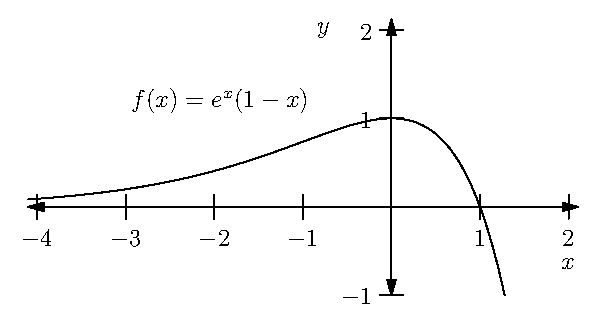
\includegraphics[width=0.55\textwidth]{nm_func_1.eps}
\end{wrapfigure}
Consider the function
  \begin{equation*}
    f(x)=e^x(1-x)
  \end{equation*}
  Show that this function has a root at $x=1$. Comment on using Newton's method to estimate this root using the initial guesses ${-1,0,1,2}$.
\\
\begin{enumerate}
\setcounter{enumi}{3}
\item%
  By considering the inverse problem, use Newton's method to estimate $\cosh^{-1}(2)$ using an initial guess of $\cosh^{-1}(2)\cong 1$. Note that the derivative of $\cosh(x)$ is $\sinh(x)$. Stop when the $\cosh$ of your estimate is within $0.001$ of $2$.

\item
  Given $f(x)=\tan^{-1}(x)$ and $f'(x)=\frac{1}{1+x^2}$, use Newton's method to estimate the root of $f$ using the following initial estimates and comment on the results.
  \begin{multicols}{3}
    \begin{enumerate}
      \item $x_0=0$ \item $x_0=1$ \item $x_0=2$ 
    \end{enumerate}
  \end{multicols}
\end{enumerate}


\end{document}

%%% Local Variables: 
%%% mode: latex
%%% TeX-master: t
%%% End: 
